\chapter{Bibliographie et Analyse}
\label{cp:bibliographie}

\section{IMU}

\paragraph{Un IMU (Inertial Measurement Unit) est un dispositif électronique qui mesure et rapporte les données d'accélération linéaire, de vitesse angulaire et d'orientation d'un objet. Les IMU sont largement utilisés dans les applications de navigation inertielle, de robotique et de réalité virtuelle.}

\paragraph{Les IMU sont généralement composés de trois capteurs principaux : un accéléromètre, un gyroscope et un magnétomètre. L'accéléromètre mesure l'accélération linéaire de l'objet, le gyroscope mesure la vitesse angulaire de l'objet et le magnétomètre mesure le champ magnétique terrestre pour déterminer l'orientation de l'objet.}

\paragraph{Les IMU sont souvent utilisés en combinaison avec d'autres capteurs, tels que les GPS et les caméras, pour fournir des données de localisation et d'orientation plus précises. Les IMU sont également utilisés dans les applications de réalité virtuelle pour suivre les mouvements de la tête de l'utilisateur et fournir une expérience immersive.}

\begin{figure}[!htpb]
    \centering
    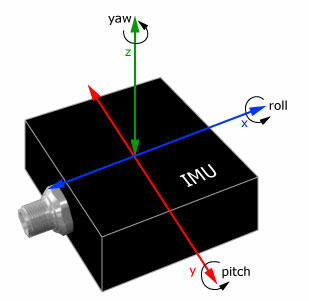
\includegraphics[width=0.5\linewidth]{Figures/imu.jpg}
    \caption[Schéma d'un IMU]{Schéma d'un IMU.}
    \label{fig:imu}
\end{figure}

\subsection{MPU6050}

\paragraph{Le MPU6050 est un IMU à 6 axes qui combine un accéléromètre et un gyroscope dans un seul boîtier. Le MPU6050 est largement utilisé dans les applications de robotique et de contrôle de mouvement en raison de sa petite taille, de sa faible consommation d'énergie et de sa précision élevée. Le MPU6050 est capable de mesurer l'accélération linéaire dans les trois axes et la vitesse angulaire dans les trois axes. Il put communiquer avec un microcontrôleur en utilisant le protocole \gls{i2c} ou \gls{spi}.}

\paragraph*{}
\begin{figure}[!htpb]
    \centering
    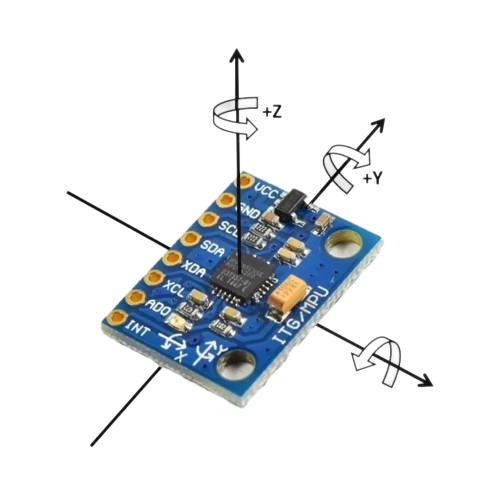
\includegraphics[width=0.8\linewidth]{Figures/mpu6050.png}
    \caption[Module MPU6050]{Module MPU6050.}
    \label{fig:mpu-6050}
\end{figure}


\subsection{I2C}

\paragraph{L'\gls{i2c} est un bus de communication série d'architecture Maitre-esclaves qui permet à plusieurs périphériques de communiquer entre eux à l'aide d'un seul bus de données. L'I2C est largement utilisé dans les applications de capteurs et de contrôleurs pour connecter plusieurs périphériques à un microcontrôleur.}

\paragraph{L'I2C utilise deux fils pour la communication : un fil de données (\acrshort{sda}) et un fil d'horloge (\acrshort{scl}). Chaque périphérique connecté au bus I2C possède une adresse unique qui lui permet de communiquer avec les autres périphériques sur le bus. L'I2C prend en charge plusieurs vitesses de communication, allant de 100 kHz à 3,4 MHz.}

\paragraph*{}
\begin{figure}[!htpb]
	\centering
	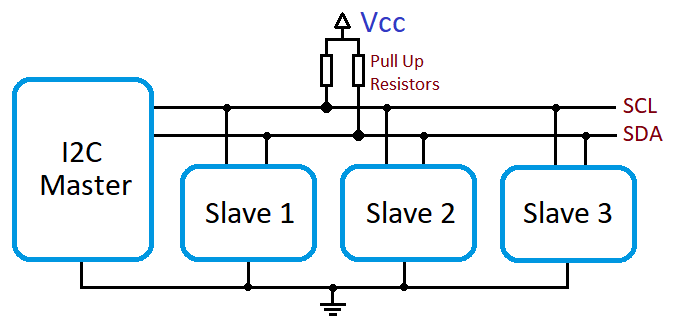
\includegraphics[width=\linewidth]{Figures/i2c.png}
	\caption[Schéma d'un bus I2C]{Schéma d'un bus I2C.}
	\label{fig:i2c}
\end{figure}

\subsection{Paquet I2C}

\paragraph{Un paquet I2C est composé de :}

\begin{enumerate}
	\item \textbf{Condition de demarage :} Un signal de valeur haute sur \acrshort{sda} et \acrshort{scl} indique le début de la communication.
	\item \textbf{Adresse client :} L'adresse du périphérique esclave auquel le maître souhaite communiquer.
	\item \textbf{Ecriture/Lecture :} Un bit de lecture/écriture indique si le maître souhaite lire ou écrire des données. (R = 1, W = 0)
	\item \textbf{Acknowledge :} Un bit de valeur basse sur \acrshort{sda} indique que le périphérique esclave a reçu les données avec succès.
	\item \textbf{Données :} Les données à écrire ou lire.
	\item \textbf{Acknowledge :} Un bit de valeur basse sur \acrshort{sda} indique que le périphérique esclave a reçu les données avec succès.
	\item \textbf{Condition d'arrêt :} Un signal de valeur basse sur \acrshort{sda} et haute sur \acrshort{scl} indique la fin de la communication.
\end{enumerate}

\paragraph*{\textbf{Adresse client} est composé de 7 bits d'adresse et d'un bit de lecture/écriture. Alors que \textbf{les paquets de données} peuvent etre sequentiels composés de 8 bits de données et un bit d'acknowledge entre eux.}

\begin{figure}[!htpb]
	\centering
	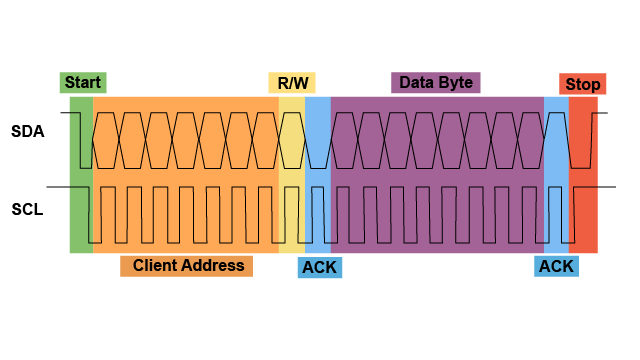
\includegraphics[width=\linewidth]{Figures/i2c-packet.png}
	\caption[Paquet I2C]{Paquet I2C.}
	\label{fig:i2c-packet}
\end{figure}

\section{Calcul de l'orientation}

\paragraph{Il existe plusieurs méthodes pour calculer l'orientation d'un objet à partir des données d'un IMU. Les méthodes les plus courantes sont les filtres de Kalman, les filtres de Mahony et les filtres de Madgwick. Ces filtres utilisent les données de l'accéléromètre, du gyroscope (et du magnétomètre facultatif mais reduit la marge de l'erreur) pour estimer l'orientation de l'objet en temps réel.}

\subsubsection{Les Angles d'Euler}

\paragraph{Les angles d'Euler sont une méthode courante pour représenter l'orientation d'un objet dans l'espace tridimensionnel. Les angles d'Euler sont composés de trois angles : l'angle de roulis, l'angle de tangage et l'angle de lacet. Ces angles décrivent la rotation de l'objet autour de ses axes X, Y et Z respectivement d'un système de coordonnées fixe.}


\begin{enumerate}
	\item \textbf{Roulis (Roll) :} Rotation autour de l'axe X. $\theta$.
	\item \textbf{Tangage (Pitch) :} Rotation autour de l'axe Y. $\phi$.
	\item \textbf{Lacet (Yaw) :} Rotation autour de l'axe Z. $\psi$.
\end{enumerate}

\pagebreak

\subsubsection{La matrice de rotation}

\begin{equation*}
	R_x = \begin{bmatrix}
		1 & 0 & 0 \\
		0 & \cos(\theta) & -\sin(\theta) \\
		0 & \sin(\theta) & \cos(\theta)
	\end{bmatrix}
\end{equation*}

\begin{equation*}
	R_y = \begin{bmatrix}
		\cos(\phi) & 0 & \sin(\phi) \\
		0 & 1 & 0 \\
		-\sin(\phi) & 0 & \cos(\phi)
	\end{bmatrix}
\end{equation*}

\begin{equation*}
	R_z = \begin{bmatrix}
		\cos(\psi) & -\sin(\psi) & 0 \\
		\sin(\psi) & \cos(\psi) & 0 \\
		0 & 0 & 1
	\end{bmatrix}
\end{equation*}

\begin{equation*}
	R_{xyz} = R_x(\theta) \times R_y(\phi) \times R_z(\psi)
\end{equation*}

\begin{equation*}
	R_{xyz} = \begin{bmatrix}
		\cos(\phi) \cos(\psi) & \cos(\phi) \sin(\psi) & -\sin(\phi) \\
		\sin(\theta) \sin(\phi) \cos(\psi) - \cos(\theta) \sin(\psi) & \sin(\theta) \sin(\phi) \sin(\psi) + \cos(\theta) \cos(\psi) & \sin(\theta) \cos(\phi) \\
		\cos(\theta) \sin(\phi) \cos(\psi) + \sin(\theta) \sin(\psi) & \cos(\theta) \sin(\phi) \sin(\psi) - \sin(\theta) \cos(\psi) & \cos(\theta) \cos(\phi)
	\end{bmatrix}
\end{equation*}

\paragraph{On définit la matrice R de rotation du capteur par rapport au repère fixe.}

\begin{equation}
	R = R_{xyz}
\end{equation}

\subsection{Accéléromètre}


\subsubsection{Modèle Mathématique}

\paragraph{L'accélération linéaire mesurée par l'accéléromètre est composée, l'accélération gravitationnelle et de l'accélération linéaire de l'objet, le biais de l'accéléromètre et le bruit de l'accéléromètre.}

\begin{equation}
	\vec{a} = \frac{\vec{dv}}{dt} - R * \vec{g} + b_a(t) + n_a(t)
\end{equation}

\begin{itemize}
	\item $\vec{a}$ est l'accélération linéaire mesurée par l'accéléromètre.
	\item $R$ est la matrice de rotation du capteur.
	\item $b_a(t)$ est le biais de l'accéléromètre.
	\item $n_a(t)$ est le bruit de l'accéléromètre.
\end{itemize}

\paragraph{L'accélération gravitationnelle est définie comme :}
\begin{equation*}
	g = 9.81 \, m/s^2
\end{equation*}

\begin{equation*}
	g = 1 gram\\
\end{equation*}

\paragraph*{Pour une plage de mesure de l'accéléromètre de $\pm 4g$ on a :}

\begin{equation*}
	g = \frac{2^{16}}{8grams} * 1gram = 8192\hspace*{.2cm}(raw\hspace*{.1cm}sensor)
\end{equation*}



\paragraph{Dans un premier temps on se pose au repos donc l'accélération linéaire est nulle aussi nous allons négliger le bruit et le biais de l'accéléromètre pour simplifier le modèle.}

\begin{equation*}
	\vec{a} = -R * \vec{g}
\end{equation*}

\paragraph{On deduit trois equations pour les trois axes de l'accéléromètre.}

\begin{align*}
	a_x &= g \sin(\phi) \\
	a_y &= -g \sin(\theta) \cos(\phi)\\
	a_z &= -g \cos(\theta) \cos(\phi)
\end{align*}

\paragraph{Pour ce projet notre bras posede un seul degré de liberté, donc nous allons utiliser l'angle de tangage pour déterminer la position du bras.}


\begin{equation}
	\hat{\phi}_{accelo}(n) = \arcsin\left(\frac{a_x(n)}{g}\right)
\end{equation}

\paragraph{}
\subsection{Gyroscope}

\paragraph{L'intégrale de la rotation est une méthode simple pour estimer l'orientation d'un objet à partir des données d'un gyroscope. L'intégrale de la rotation consiste à intégrer les données du gyroscope pour estimer l'orientation de l'objet en temps réel.}

\subsubsection{Modèle Mathématique}

\paragraph{La vitesse angulaire mesurée par le gyroscope est composée de la vitesse angulaire de l'objet, du biais du gyroscope et du bruit du gyroscope.}

\begin{equation}
	\omega = \frac{d\phi}{dt} + b_g(t) + n_g(t)
\end{equation}

\begin{enumerate}
	\item $\omega$ est la vitesse angulaire mesurée par le gyroscope.
	\item $\frac{d\phi}{dt}$ est la vitesse angulaire reelle.
	\item $b_g(t)$ est le biais du gyroscope.
	\item $n_g(t)$ est le bruit du gyroscope.
\end{enumerate}

\paragraph{De meme on neglige le bruit et le biais du gyroscope pour simplifier le modèle.}
\begin{equation}
	\hat{\phi}_{gyro}(n) =  \int_{0}^{n*T} \dot{\phi}(n) \,dt
\end{equation}

\begin{equation}
	\hat{\phi}_{gyro}(n) =  \sum_{i=0}^{n} \dot{\phi}(i) * T
\end{equation}

\begin{itemize}
	\item $\hat{\phi}_{gyro}(n)$ est l'angle de tangage estimé à partir des données du gyroscope.
	\item $\dot{\phi}(i)$ est la vitesse angulaire du gyroscope à l'instant i.
	\item $T$ est l'intervalle de temps entre deux mesures.
\end{itemize}

\paragraph{Le problème de cette estimation de l'orientation à partir du gyroscope est la dérive du gyroscope. L'erreur cumulée de l'intégration des données du gyroscope entraîne une dérive de l'angle de tangage au fil du temps.}
\paragraph*{}
\begin{figure}[!htpb]
	\centering
	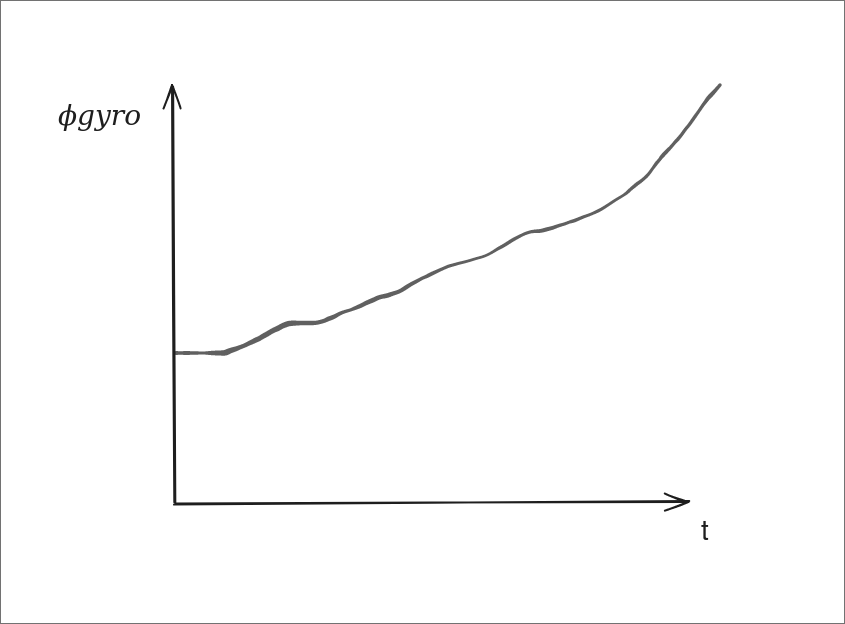
\includegraphics[width=0.7\linewidth]{Figures/drift.png}
	\caption[Dérive du gyroscope]{Dérive du gyroscope.}
\end{figure}

\paragraph{Le modèle mathématique le plus proche de la réalité est le suivant :}

\begin{equation}
	\phi(n) = \int_{0}^{n*T} (\dot{\phi} + b_{\phi}(t) + n_{\phi}(t)) \,dt
\end{equation}

\begin{itemize}
	\item $\phi(n)$ est l'angle de tangage réel.
	\item $\dot{\phi}$ est la vitesse angulaire réelle.
	\item $b_{\phi}(t)$ est le biais de l'angle de tangage suit une loi normale.
	\item $n_{\phi}(t)$ est le bruit de l'angle de tangage suit une loi normale.
\end{itemize}


\subsection{Filtre complémentaire}

\paragraph{Le filtre complémentaire est une méthode courante pour estimer l'orientation d'un objet à partir des données d'un IMU. Le filtre complémentaire combine les données de l'accéléromètre et du gyroscope pour estimer l'orientation de l'objet en temps réel.}

\paragraph{Apres avoir calculé l'angle de tangage à partir des données de l'accéléromètre et du gyroscope, on peut combiner ces deux estimations en utilisant un filtre complémentaire pour obtenir une estimation plus précise de l'orientation de l'objet.}

\begin{equation}
	\hat{\phi}(n) = \alpha * \hat{\phi}_{gyro}(n) + (1 - \alpha) * \hat{\phi}_{accelo}(n)
\end{equation}

\begin{itemize}
	\item \textbf{$\alpha$ :} compis entre 0 et 1 est un paramètre de pondération qui détermine la contribution de chaque estimation à l'orientation finale de l'objet.
\end{itemize}


\paragraph{
	Le gyroscope donne l'estimation de l'angle mais il est sujet à la dérive, tandis que l'accéléromètre donne une estimation stable mais sujette aux vibrations. Ce filtre complémentaire compense la derive du gyroscope en utilisant l'accéléromètre pour obtenir une estimation plus précise de l'orientation de l'objet.
}

\section{Filtre de Madgwick}

\paragraph{Le filtre de Madgwick est une méthode courante et la meilleure pour estimer l'orientation d'un objet à partir des données d'un IMU. Le filtre de Madgwick utilise les données de l'accéléromètre, du gyroscope et du magnétomètre (facultatif mais peut minimiser l'erreur) pour estimer l'orientation de l'objet en temps réel.}

\paragraph{Le filtre de Madgwick utilise un algorithme de filtrage basé sur les quaternions pour estimer l'orientation de l'objet. Les quaternions sont une méthode mathématique pour représenter l'orientation d'un objet dans l'espace tridimensionnel. Les quaternions sont composés de quatre valeurs : un scalaire et un vecteur.}

\begin{equation}
	\mathbf{q}_{\omega, t}=\begin{bmatrix}q_w & q_x & q_y & q_z\end{bmatrix}
\end{equation}

\begin{itemize}
	\item $q_w$ est le scalaire.
	\item $q_x, q_y, q_z$ sont les composantes du vecteur.
\end{itemize}

\paragraph{Le filtre utilise une représentation quaternionique de l'orientation pour décrire la nature des orientations en trois dimensions et n'est pas soumis aux singularités associées à une représentation par angles d'Euler, permettant d'utiliser les données de l'accéléromètre et du magnétomètre dans un algorithme de descente de gradient dérivé analytiquement et optimisé pour calculer la direction de l'erreur de mesure du gyroscope en tant que dérivée quaternionique.}

\begin{equation}
	\begin{split}\begin{array}{rcl}
		\mathbf{q}_{\omega, t} &=& \,\mathbf{q}_{t-1} + \,\dot{\mathbf{q}}_{\omega, t}\Delta t\\
		&=& \,\mathbf{q}_{t-1} + \frac{1}{2}\big(\,\mathbf{q}_{t-1}\mathbf{\,^I\omega_t}\big)\Delta t
	\end{array}\end{split}
\end{equation}


\begin{itemize}
	\item $\dot{q}$ est la dérivée du quaternion.
	\item $\omega$ est la vitesse angulaire mesurée par le gyroscope.
	\item $\Delta t$ est l'intervalle de temps entre deux mesures.
\end{itemize}

\paragraph{Orientation en tant que solution de la descente de gradient}

\paragraph{Le filtre Madgwick formule le problème d'estimation d'attitude dans l'espace quaternionique. L'idée générale du filtre Madgwick est d'estimer q en fusionnant/combinant les estimations d'attitude par l'intégration des mesures du gyroscope $\omega$ et la direction obtenue par les mesures de l'accéléromètre a. En essence, les estimations d'attitude du gyroscope sont utilisées comme des représentations précises sur de courtes périodes de temps et pour des mouvements rapides, tandis que les estimations d'attitude de l'accéléromètre sont utilisées comme des directions précises pour compenser la dérive à long terme du gyroscope par intégration.}

\paragraph{Ainsi, la fonction objective est :}
\begin{equation}
	f\left({}^{I}_{W}\mathbf{\hat{q}}, {}^{W}\mathbf{\hat{g}}, {}^{I}\mathbf{\hat{a}}  \right)  = {}^{I}_{W}\mathbf{\hat{q^*}} \otimes {}^{W}\mathbf{\hat{g}} \otimes {}^{I}_{W}\mathbf{\hat{q}} - {}^{I}\mathbf{\hat{a}}
\end{equation}

\begin{itemize}
	\item $q^*$ est le conjugué du quaternion.
	\item $a$ est l'accélération linéaire mesurée par l'accéléromètre.
	\item $g$ est l'accélération gravitationnelle.
\end{itemize}

\paragraph{La solution de ce problème d'optimisation est la direction de l'erreur de mesure du gyroscope.}

\begin{equation}
	\min_{{}^{I}_{W}\mathbf{\hat{q}} \in \mathbb{R}^{4 \times 1} } f\left({}^{I}_{W}\mathbf{\hat{q}}, {}^{W}\mathbf{\hat{g}}, {}^{I}\mathbf{\hat{a}} \right)
\end{equation}

\paragraph{L'approche suggérée de cet estimateur est d'utiliser l'algorithme de descente de gradient pour calculer la solution.}

\paragraph{À partir d'une estimation initiale $q_0$ et d'une taille de pas $\beta$, l'algorithme de descente de gradient pour N itérations, qui estime les orientations $q_i$, est décrit comme suit :}

\begin{equation}
	{}^{I}_{W}\mathbf{q}_{\nabla, t+1} = - \beta\frac{\nabla f\left( {}^{I}_{W}\mathbf{\hat{q}}_{est, t}, {}^{W}\mathbf{\hat{g}}, {}^{I}\mathbf{\hat{a}}_{t+1} \right)}{\vert \vert  \nabla f\left( {}^{I}_{W}\mathbf{\hat{q}}_{est, t}, {}^{W}\mathbf{\hat{g}}, {}^{I}\mathbf{\hat{a}}_{t+1} \right) \vert \vert}\end{equation}


\begin{itemize}
	\item $\beta$ est le pas de la descente de gradient.
	\item $\nabla f$ est le gradient de la fonction objective.
	\item $\|\nabla f\|$ est la norme du gradient.
\end{itemize}

\subsection{Etape 1: obtenir les données des capteurs}

\paragraph{Obtenez les mesures du gyroscope et de l'accéléromètre à partir du capteur. Soit ${}^I\omega_t$ et ${}^I\mathbf{a}_t$ les mesures du gyroscope et de l'accéléromètre respectivement. De plus, ${}^I\mathbf{a}_t$ désigne les mesures de l'accéléromètre normalisées.}

\subsection{Etape 2: Incrementation d'orientation par l'accéléromètre}

\paragraph{Calculez l'incrément d'orientation à partir des mesures de l'accéléromètre (étape de gradient).}

\begin{equation}
	\nabla f\left( {}^{I}_{W}\mathbf{\hat{q}}_{est, t}, {}^{W}\mathbf{\hat{g}}, {}^{I}\mathbf{\hat{a}}_{t+1} \right) =  J^T\left( {}^{I}_{W}\mathbf{\hat{q}}_{est, t}, {}^{W}\mathbf{\hat{g}} \right) f\left( {}^{I}_{W}\mathbf{\hat{q}}_{est, t}, {}^{W}\mathbf{\hat{g}}, {}^{I}\mathbf{\hat{a}}_{t+1} \right)
\end{equation}

\begin{equation}
	f\left( {}^{I}_{W}\mathbf{\hat{q}}_{est, t}, {}^{W}\mathbf{\hat{g}}, {}^{I}\mathbf{\hat{a}}_{t+1} \right) = \begin{bmatrix}  
		2\left( q_2q_4 - q_1q_3\right) - a_x\\
		2\left( q_1q_2 + q_3q_4\right) - a_y\\
		2\left( \frac{1}{2} - q_2^2 - q_3^2\right) - a_z\\
		\end{bmatrix}
\end{equation}

\begin{equation}
	J\left( {}^{I}_{W}\mathbf{\hat{q}}_{est, t}, {}^{W}\mathbf{\hat{g}} \right) = \begin{bmatrix}  
		-2q_3 & 2q_4 & -2q_1 & 2q_2 \\
		2q_2 & 2q_1 & 2q_4 & 2q_3 \\
		0 & -4q_2 & -4q_3 & 0\\
		\end{bmatrix}
\end{equation}

\paragraph{Mettre a jour le terme (composante d'attitude à partir des mesures de l'accéléromètre) est donné par}

\begin{equation}
	{}^{I}_{W}\mathbf{q}_{\nabla, t+1} = - \beta\frac{\nabla f\left( {}^{I}_{W}\mathbf{\hat{q}}_{est, t}, {}^{W}\mathbf{\hat{g}}, {}^{I}\mathbf{\hat{a}}_{t+1} \right)}{\vert \vert  \nabla f\left( {}^{I}_{W}\mathbf{\hat{q}}_{est, t}, {}^{W}\mathbf{\hat{g}}, {}^{I}\mathbf{\hat{a}}_{t+1} \right) \vert \vert}
\end{equation}

\subsection{Etape 3: Mise à jour de l'orientation par le gyroscope}

\paragraph{Calculez l'incrément d'orientation à partir des mesures du gyroscope (étape d'intégration).}

\begin{equation}
	{}^{I}_{W}\dot{\mathbf{q}}_{\omega,t+1} = \frac{1}{2} {}^{I}_{W}\hat{\mathbf{q}}_{est,t}\otimes \begin{bmatrix} 0, {}^{I}\omega_{t+1} \end{bmatrix}^T
\end{equation}

\subsection{Etape 4: Fusion des mesures}

\paragraph{Fusionnez les mesures du gyroscope et de l'accéléromètre pour obtenir l'orientation estime finale.}

\begin{equation}
	{}^{I}_{W}\dot{\mathbf{q}}_{est, t+1} = {}^{I}_{W}\dot{\mathbf{q}}_{\omega, t+1} + {}^{I}_{W}\mathbf{q}_{\nabla, t+1}
\end{equation}

\begin{equation}
	{}^{I}_{W}\mathbf{q}_{est, t+1} = {}^{I}_{W}\hat{\mathbf{q}}_{est, t} + {}^{I}_{W}\mathbf{\dot{q}}_{est, t+1} \Delta t
\end{equation}

\paragraph{Ici, $\Delta t$ représente le temps écoulé entre deux échantillons à $t$ et $t+1$.}

\subsection{Derniere etape}

\paragraph{Répétez les étapes 1 à 4 pour chaque échantillon de données pour obtenir l'orientation estimée en temps réel.}

\section{ESC}

\paragraph{Un ESC (Electronic Speed Controller) est un dispositif électronique qui convertie DC/AC (DAC) et contrôle la vitesse d'un moteur électrique en ajustant la tension et le courant fournis au moteur. Les ESC sont largement utilisés dans les applications de robotique, de drones et de modélisme pour contrôler la vitesse des moteurs électriques.}

\paragraph{On peut controler la vitesse d'un moteur électrique en ajustant la tension et le courant fournis au moteur. pour varier cette derniere on utilise un signal \acrshort{pwm} (Pulse Width Modulation) qui permet de controler la vitesse du moteur en ajustant la largeur des impulsions du signal.}

\begin{figure}[!htpb]
	\centering
	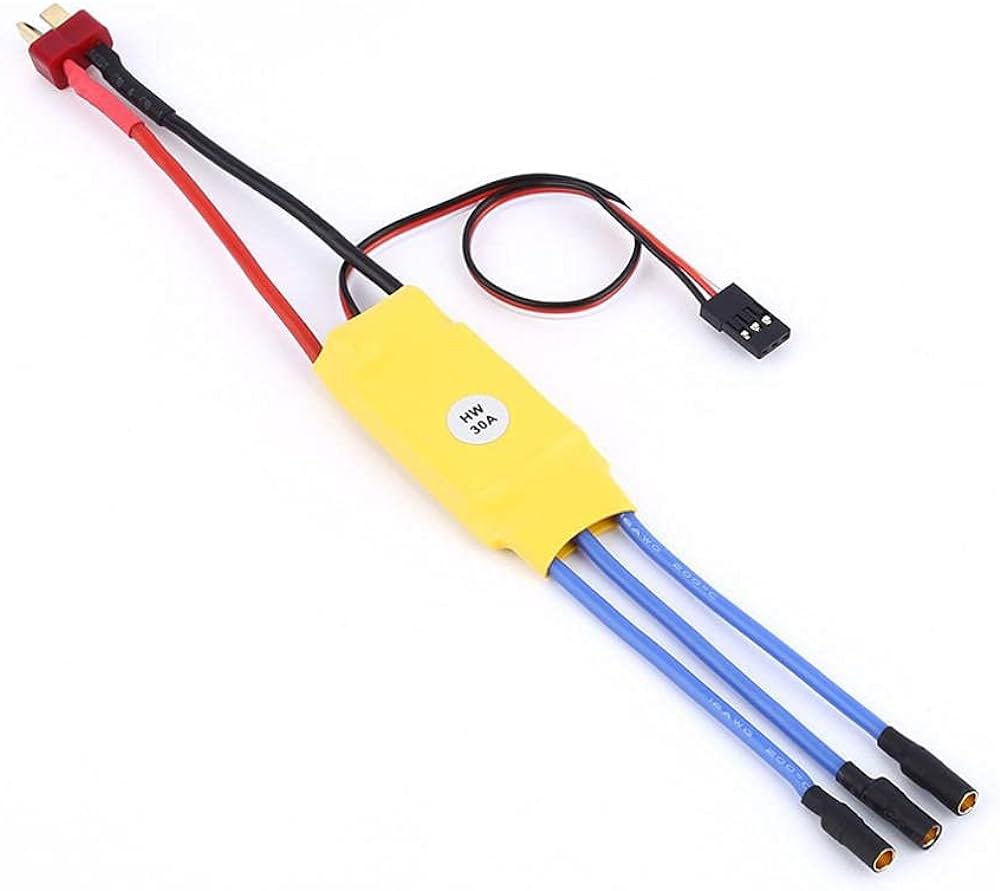
\includegraphics[width=0.7\linewidth]{Figures/esc.jpg}
	\caption[ESC]{ESC.}
\end{figure}

\paragraph{
	On alimente l'ESC avec une tension continue de 5V à 12V, et on controle la vitesse du moteur en ajustant la largeur des impulsions du signal PWM. La largeur de l'impulsion determine la vitesse du moteur, plus l'impulsion est longue, plus la vitesse du moteur est élevée. L'ESC convertit le signal PWM en tension et courant pour controler la vitesse du moteur.
}

\begin{itemize}
	\item $T_{on} = T * \alpha$ est la relation du rapport cyclique du signal PWM.
\end{itemize}

\begin{equation}
	1000\mu s \leq T_{on} \leq 2000\mu s
\end{equation}

\subsection{Moteur A2212/13T}

\paragraph{Le moteur A2212/13T est un moteur brushless qui est largement utilisé dans les applications de drone et de modélisme. Le moteur A2212/13T est un moteur à aimant permanent qui utilise un contrôleur électronique (ESC) pour contrôler la vitesse du moteur.}

\begin{figure}[!htpb]
	\centering
	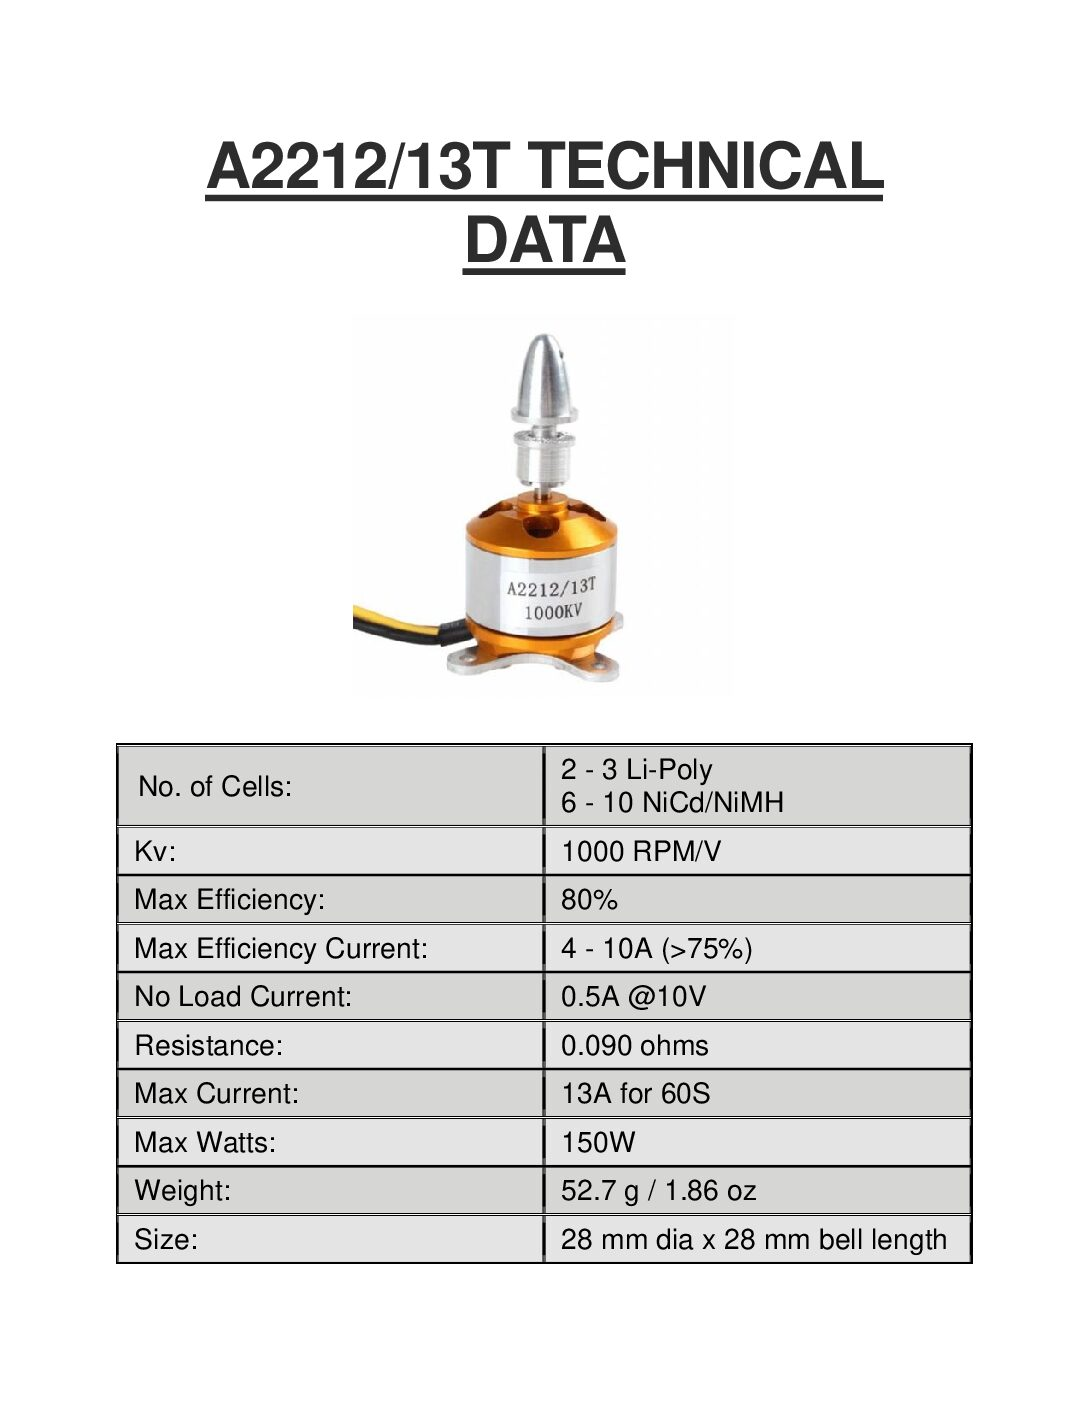
\includegraphics[width=\linewidth]{Figures/motor.jpg}
	\caption[Moteur A2212/13T]{Moteur A2212/13T.}
\end{figure}

\newpage

\subsection{Contrôle PID}

\paragraph{Le contrôle PID (Proportionnel, Intégral, Dérivé) est une méthode courante pour contrôler les systèmes dynamiques en utilisant un retour d'information. Le contrôle PID utilise trois termes pour ajuster la commande du système en fonction de l'erreur, de l'intégrale de l'erreur et de la dérivée de l'erreur.}

\paragraph{Le terme proportionnel ajuste la commande en fonction de l'erreur actuelle, le terme intégral ajuste la commande en fonction de l'accumulation de l'erreur passée et le terme dérivé ajuste la commande en fonction de la variation de l'erreur. Le contrôle PID est largement utilisé dans les applications de contrôle de mouvement, de robotique et de systèmes de contrôle automatique.}

\begin{equation}
	u(t) = K_p e(t) + K_i \int_{0}^{t} e(\tau) \,d\tau + K_d \frac{de(t)}{dt}
\end{equation}

\begin{itemize}
	\item $u(t)$ est la commande du système.
	\item $e(t)$ est l'erreur du système.
	\item $K_p, K_i, K_d$ sont les coefficients du contrôleur PID.
	\item $t$ est le temps.
	\item $\tau$ est le temps de l'intégrale.
	\item $de(t)/dt$ est la dérivée de l'erreur.
	\item $\int_{0}^{t} e(\tau) \,d\tau$ est l'intégrale de l'erreur.
\end{itemize}

\begin{figure}[!htpb]
	\centering
	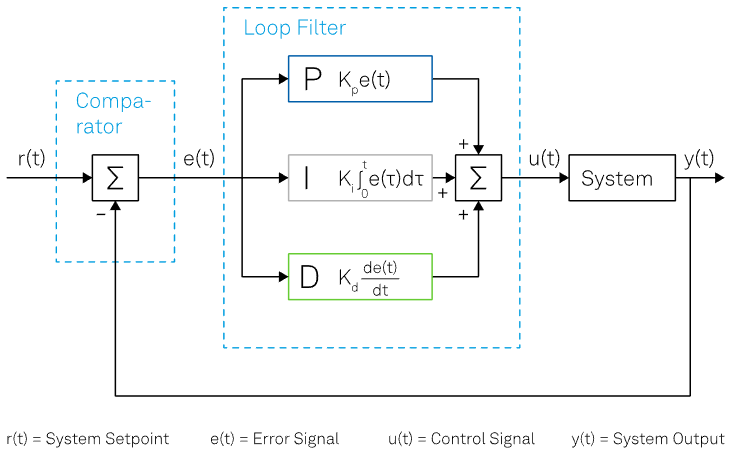
\includegraphics[width=\linewidth]{Figures/pid.png}
	\caption[Contrôle PID]{Contrôle PID.}	
\end{figure}
